%\chapter*{Anhang}
\listofappendices
\label{cha:anh}
\addcontentsline{toc}{chapter}{Anhang}
\captionsetup{list=false}




%Anhangsverzeichnis.\\\\
%\listofappendix



\clearpage

\section*{Klassen des Ausleseprogrammes}\appcaption{\hspace{-5mm}Anhang 1: Klassen des Ausleseprogrammes}
%\addcontentsline{anhang}{Klassen des Ausleseprogrammes}
%\addappendix{Klassen des Ausleseprogrammes}
%\myappendix{Klassen des Ausleseprogrammes}
\label{sec:anh:class}

In den nachfolgenden Abbildungen sind die verschiedenen Klassen des Ausleseprogrammes zu sehen, auf die im Kapitel \ref{subsec:classdiagrams} eingegangen wird.\\\\

\begin{figure}[H]
\centering
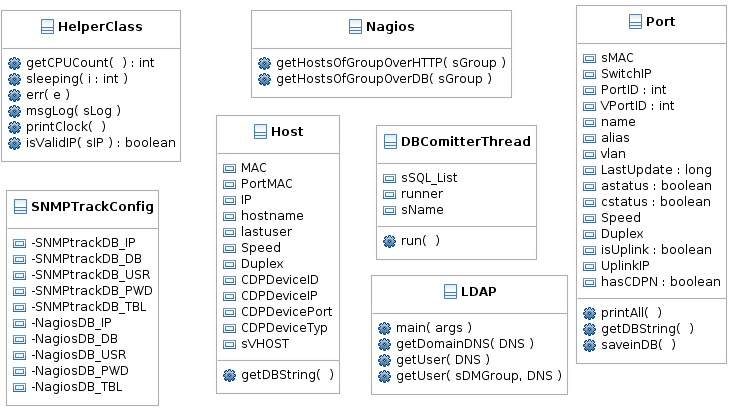
\includegraphics[width=1.0\textwidth]{model1.png}
\caption[]{Klassendiagramm}
\label{fig:classdia1}
\end{figure}

\begin{figure}[H]
\centering
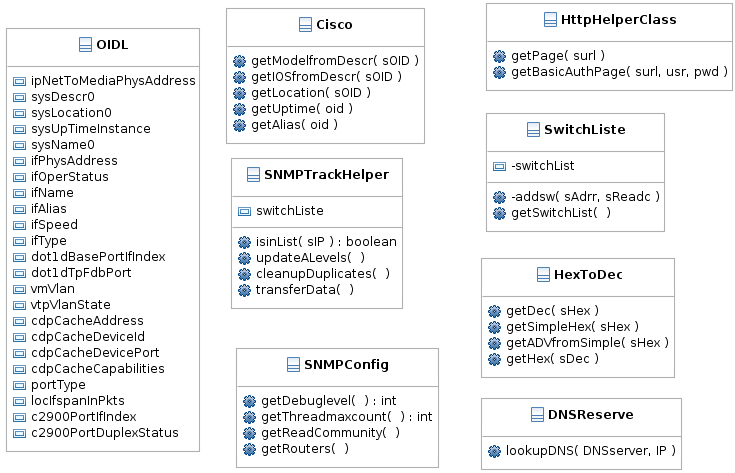
\includegraphics[width=1.0\textwidth]{model2.png}
\caption[]{Klassendiagramm}
\label{fig:classdia2}
\end{figure}

\begin{figure}[H]
\centering
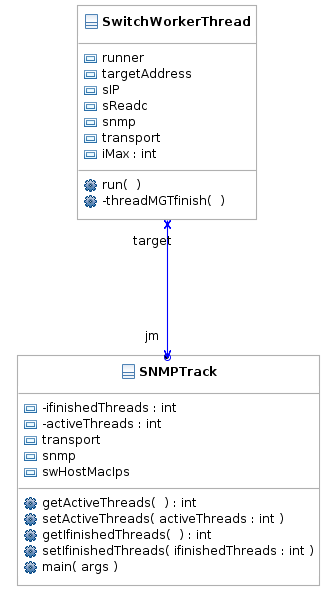
\includegraphics[width=0.4\textwidth]{model3.png}
\caption[]{Klassendiagramm}
\label{fig:classdia3}
\end{figure}

\begin{figure}[H]
\centering
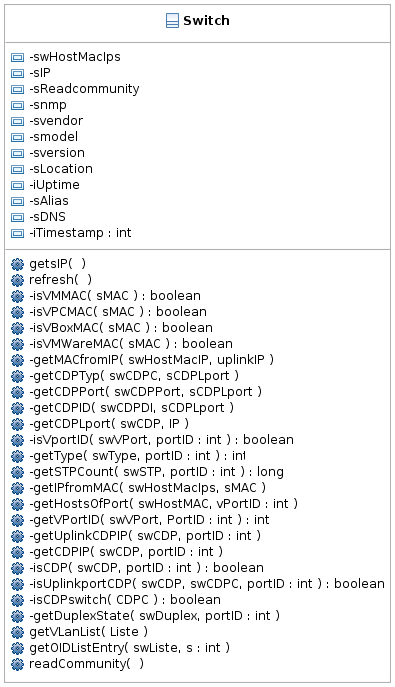
\includegraphics[width=0.6\textwidth]{model4.png}
\caption[]{Klassendiagramm}
\label{fig:classdia4}
\end{figure}

\begin{figure}[H]
\centering
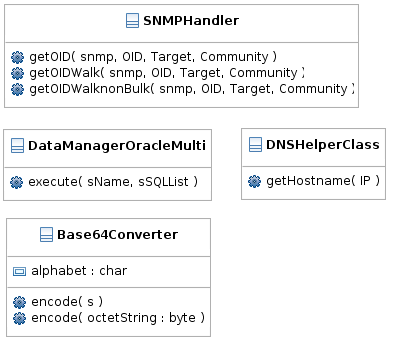
\includegraphics[width=0.6\textwidth]{model5.png}
\caption[]{Klassendiagramm}
\label{fig:classdia5}
\end{figure}

\begin{figure}[H]
\centering
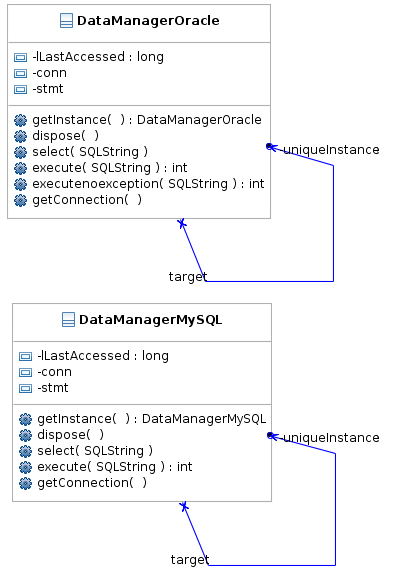
\includegraphics[width=0.6\textwidth]{model6.png}
\caption[]{Klassendiagramm}
\label{fig:classdia6}
\end{figure}

\clearpage

%\myappendix{Konfiguration SNMP-Track}
\section*{Konfiguration SNMP-Track}\appcaption{\hspace{-5mm}Anhang 2: Konfiguration SNMP-Track}
\label{sec:config}

In Abbildung \ref{fig:config_xml} ist die Konfigurations-Datei des erstellten Ausleseprogramms (SNMP-Track) zu sehen.
Diese Datei dient zur Definition der jeweiligen Datenbanken und der Parameter für SNMP-Track.
Der erste Eintrag legt die Anzahl der Threads fest. Dank einiger Optimierungen des Programms, kann dieser Wert auch über den in Kapitel \ref{sec:designent} empfohlenen Maximalwert gesetzt werden.
Jedoch ist zu beachten, dass je nach CPU-Geschwindigkeit der Switches und der Leistung des Rechners der das Ausleseprogramm ausführt es zu Engpässen kommen kann.
Der Maximalwert, der auf einem Server getestet wurde, war 128. Jedoch handelte es sich hierbei um einen Server mit einer Intel Xeon-CPU, die aus vier Cores zu je 2.8GHz besteht.\\\\

\begin{figure}[H]
\centering
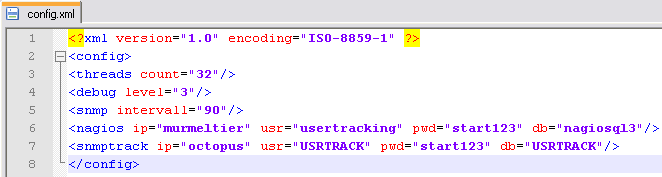
\includegraphics[width=1.0\textwidth]{config_xml.png}
\caption[]{config.xml}
\label{fig:config_xml}
\end{figure}

Der nächste Parameter legt den Debug-Level fest, der in Kapitel \ref{sec:implementation} näher beschrieben wurde.
Er dient vor allem dazu, den Detailgrad der Meldungen zu steuern.
Um die Auslesegeschwindigkeit und somit auch die Last auf den Switchs zu steuern, dient der Parameter 'SNMP Intervall'.
Dieser gibt die Zeit in ms an, die zwischen zwei SNMP Abfragen liegen soll. Ein hoher Wert führt zu geringer Last auf den Switches und einer erhöhten Auslesedauern.
Ein kleiner Wert hingegen erhöht die Last auf den Switches und reduziert die Auslesezeit.
Empfehlungswerte sind hierbei stark Geräte abhängig. Neuere Cisco Switches können problemlos mit dem Wert von 20ms arbeiten, wohingegen ältere Switches, z.B. der Catalyst 3500XL bei diesem Wert sehr stark ausgelastet ist.
Hier ist es hilfreich in den ersten Tagen des Einsatzes der Software die Last der Switches zu kontrollieren um den optimalen Wert zu finden.
Die beiden anderen Parameter stellen die Datenbanken dar, die für den Ausleseprozess benötigt werden.
Die Nagios-Datenbank dient als Quelle für die Switch-IPs und deren Hierachieebene.
Die SNMP-Datenbank enthält die Daten des Ausleseprogrammes, welche per Webinterface dargestellt werden.

\section*{Bilder der fertigen Implementierung}\appcaption{\hspace{-5mm}Anhang 3: Bilder der fertigen Implementierung}
\label{sec:impimgs}

Um einen Überblick über die implementierte Lösung zu erhalten, sind im nachfolgenden Bilder der Oberfläche zu sehen.\\\\
Die in Abbildung \ref{fig:login} zusehende Loginmaske, stellt sicher, dass nur berechtigte Personen auf die Daten der Switches zugreifne können.


\begin{figure}[H]
\centering
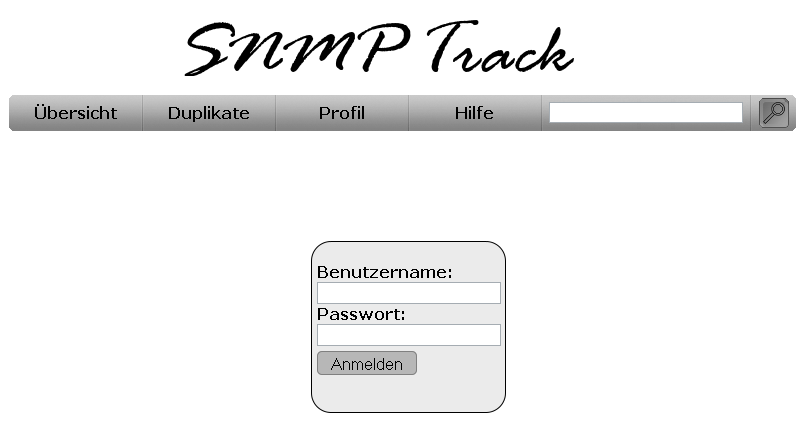
\includegraphics[width=1.0\textwidth]{login.png}
\caption[]{Weboberfläche - Login}
\label{fig:login}
\end{figure}

Nach dem Einloggen wird dem Benutzer die in Abbildung \ref{fig:overview} sichtbare Übersicht präsentiert.
Diese ermöglicht den direkten Zugriff auf die wichtigsten Funktionalitäten.
Zusätzlich wird automatisch der Cursor auf die Suchmaske gesetzt, sodass direkt per Tastatur nach dem einloggen gesucht werden kann, ohne dass der Benutzer die Maus bewegen muss.

\begin{figure}[H]
\centering
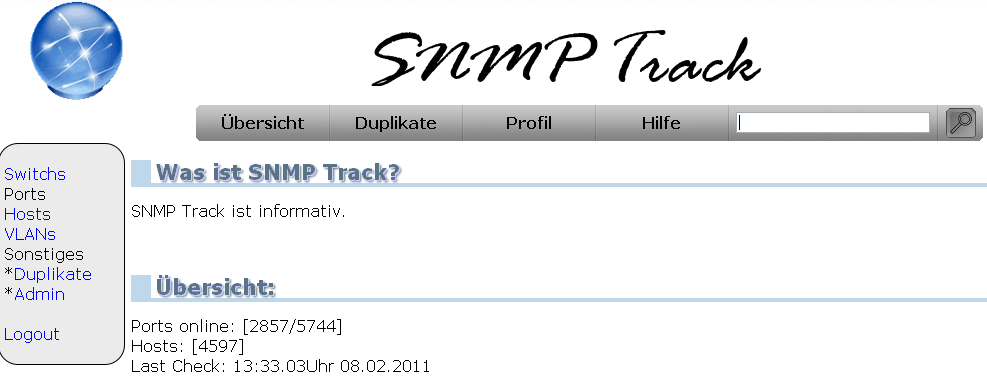
\includegraphics[width=1.0\textwidth]{overview.png}
%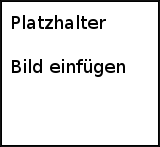
\includegraphics[width=0.5\textwidth]{000.PNG}
\caption[]{Weboberfläche - Übersicht}
\label{fig:overview}
\end{figure}

Geht der Benutzer zum Menüpunkt Switches, so erhält er eine Übersicht über die im Netzwerk auslesbaren Switches.
Diese sindin Abbildung \ref{fig:overview} zu sehen.

\begin{figure}[H]
\centering
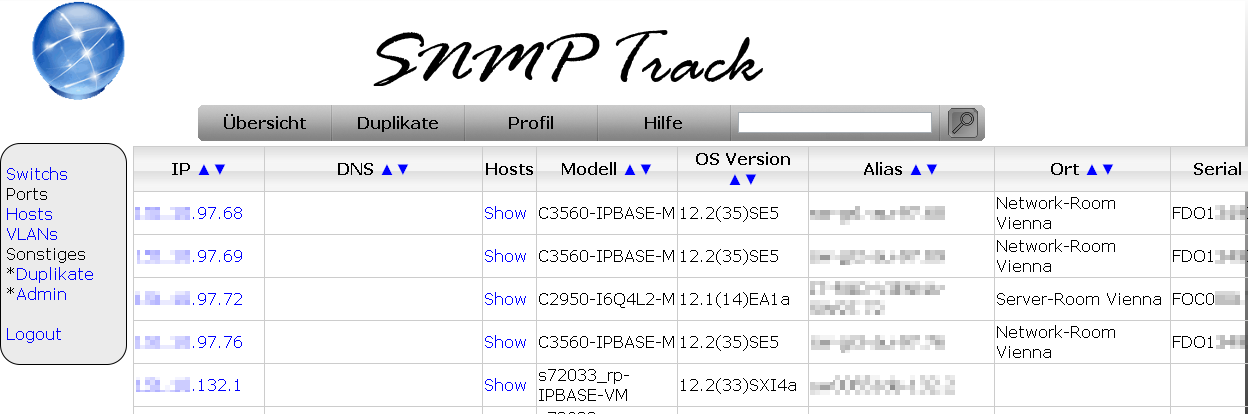
\includegraphics[width=1.0\textwidth]{switchs.png}
\caption[]{Weboberfläche - Switchs}
\label{fig:overview}
\end{figure}

Wählt der Benutzer nun einen der Switchs aus, so gelangt er auf die Übersicht der Ports, die im Switch verbaut sind.
Diese ist in Abbildung \ref{fig:overview} zu sehen.

\begin{figure}[H]
\centering
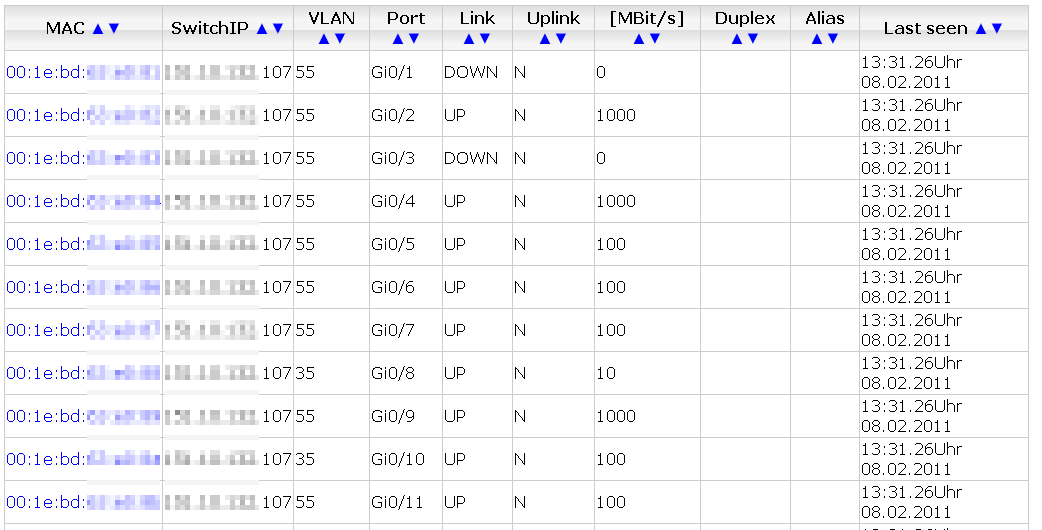
\includegraphics[width=1.0\textwidth]{ports.png}
\caption[]{Weboberfläche - Ports}
\label{fig:overview}
\end{figure}

Wenn der Benutzer nun einen der Ports selektiert hat, so kann er die hinter befindlichen Hosts in einer Liste sehen.
Neben der Übersicht der Hosts kann der Benutzer sich auch ein Überblick über die verwendeten VLANs verschaffen.
Hierzu muss nur der Menüpunkt VLANs aufgerufen werden und anschließend erhält mein die Übersicht wie in Abbildung \ref{fig:vlans} zu sehen.

\begin{figure}[H]
\centering
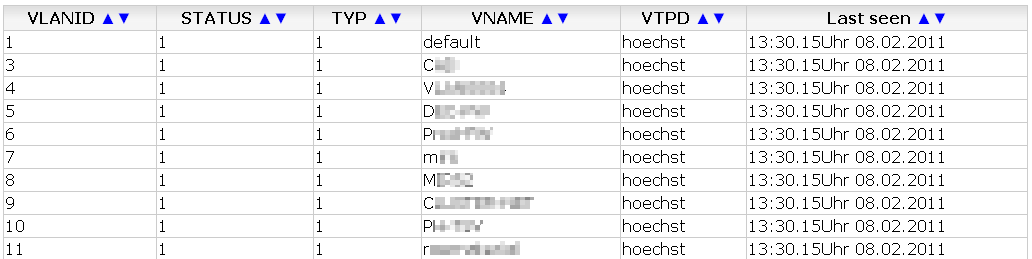
\includegraphics[width=1.0\textwidth]{vlans.png}
\caption[]{Weboberfläche - VLANs}
\label{fig:vlans}
\end{figure}

Neben der Administration der Nutzer bietet der Admin-Menüpunkt zusätzlich die Möglichkeit einen Auslese-Vorgang zu starten, wie in Abbildung \ref{fig:adminpanel} zu sehen.
Hierbei hat der Benutzer der Stufe Administrator die Wahl, ob er alle Switches, oder nur einen selektiven aktualisieren möchte.
Dies ist in der Praxis vor allem interessant, wenn man eine zeitnahe Information benötigt, die nicht im 30-Minuten Ausleseintervall liegt.
Beispielsweise befindet sich ein Benutzer auf dem Werksgelände in der Produktion und kann von dort aus manuell ein Auslesevorgang starten, um zu überprüfen, ob der Status eines Ports sich geändert hat.
Dies ist vor allem beim Patchen von Verbindungen hilfreich.

\begin{figure}[H]
\centering
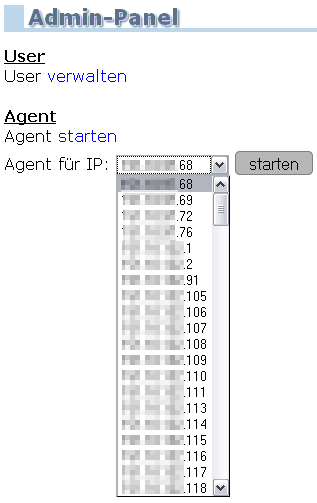
\includegraphics[width=0.5\textwidth]{admin_panel.png}
%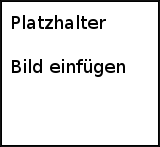
\includegraphics[width=0.5\textwidth]{000.PNG}
\caption[]{Weboberfläche - Adminpanel}
\label{fig:adminpanel}
\end{figure}

In der folgenden Abbildung \ref{fig:ausleseprogramm} ist das Ausleseprogramm zu sehen.
Diese gibt den Start des Programms wieder, wie er in Kapitel \ref{subsec:acitvitydiagrams} beschrieben ist.
Hierbei sind auch Meldungen über die ausgelesene Konfiguration zu finden.
Zuerst werden die Performance Parameter (Threadanzahl, SNMP-Intervall) sowie das Debuglevel angezeigt.
Im Anschluss wird überprüft ob die Datei switch.xml vorhanden ist und je nachdem werden die Daten aus diese oder dem Nagios-System ausgelesen.

\begin{figure}[H]
\centering
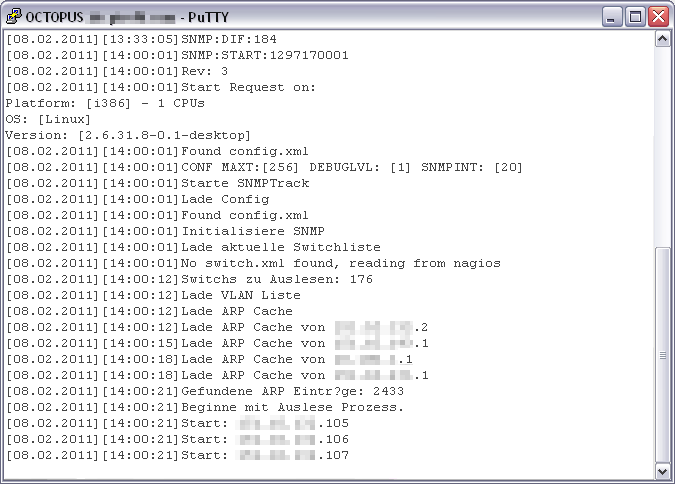
\includegraphics[width=1.0\textwidth]{ausleseprogramm.png}
\caption[]{Ausleseprogramm - Start}
\label{fig:ausleseprogramm}
\end{figure}








